\documentclass{beamer}

\usepackage[orientation=landscape,size=a0,scale=1.4,debug]{beamerposter}
\mode<presentation>{\usetheme{mlr}}

\usepackage[sfdefault]{roboto}
\usepackage{roboto-mono}
\usepackage[T1]{fontenc}
\usepackage[utf8]{inputenc} % UTF-8
\usepackage[english]{babel} % Language
\usepackage{hyperref} % Hyperlinks
\usepackage{ragged2e} % Text position
\usepackage[export]{adjustbox} % Image position
\usepackage[most]{tcolorbox} % Code boxes

\hypersetup{
    hyperfootnotes=false,
    colorlinks=true,
	linktocpage=true,
	pdfauthor={mlr-org team},
    %linkcolor=[RGB]{3,99,142}, % mlr blue
    urlcolor=[RGB]{231,138,69}
}

\title{Dataflow programming with mlr3pipelines :\,: CHEAT SHEET} % Package title in header, \, adds thin space between ::

\newlength{\columnheight} % Adjust depending on header height
\setlength{\columnheight}{84cm}

\newtcolorbox{codebox}{%
	sharp corners,
	leftrule=0pt,
	rightrule=0pt,
	toprule=0pt,
	bottomrule=0pt,
	fontupper=\robotomono\small,
	hbox}

\newtcolorbox{codeboxmultiline}[1][]{%
	sharp corners,
	leftrule=0pt,
	rightrule=0pt,
	toprule=0pt,
	bottomrule=0pt,
	fontupper=\robotomono\small,
	#1}

    \newtcolorbox{codeboxexample}[1][]{%
	sharp corners,
	leftrule=0pt,
	rightrule=0pt,
	toprule=0pt,
	bottomrule=0pt,
	fontupper=\robotomono\small,
	width=27cm,
	adjusted title=Example #1,
	fonttitle = \bfseries\Large,
	top = 0.5em}

\newtcolorbox{codeboxinline}{%
	sharp corners,
	leftrule=0pt,
	rightrule=0pt,
	toprule=0pt,
	bottomrule=0pt,
	hbox,
	nobeforeafter,
	fontupper=\robotomono\small,
	tcbox raise base}

\newcommand{\codeinline}[1]{\begin{codeboxinline}#1\end{codeboxinline}}
\newcommand{\monospace}[1]{\multido{}{#1}{\space}}

\begin{document}
\begin{frame}[fragile]{}
  \begin{columns}
    \begin{column}{.245\textwidth}
      \begin{beamercolorbox}[center]{postercolumn}
        \begin{minipage}{.98\textwidth}
          \parbox[t][\columnheight]{\textwidth}{
            \begin{myblock}{Introduction}
              % \vspace{-0.5em}
              Combine ML operations to flexible pipelines and processing graphs, which can be configured trained, resampled, tuned as any regular learner.
              % The mlr3pipelines package is an extension for the \href{https://github.com/mlr-org/mlr3}{mlr3} package and provides \codeinline{PipeOp}s (pipeline operators) which can be connected to a \codeinline{Graph} using, e.g., the \%>{}>\% operator.
              The main purpose of a \codeinline{Graph} is to build combined preprocessing and model fitting pipelines that can be used as a \codeinline{Learner}.
              % The following schematic shows a \codeinline{GraphLearner} centering and scaling features, encoding factors and imputing missing data before a \codeinline{Learner} is applied.
              \begin{center}
                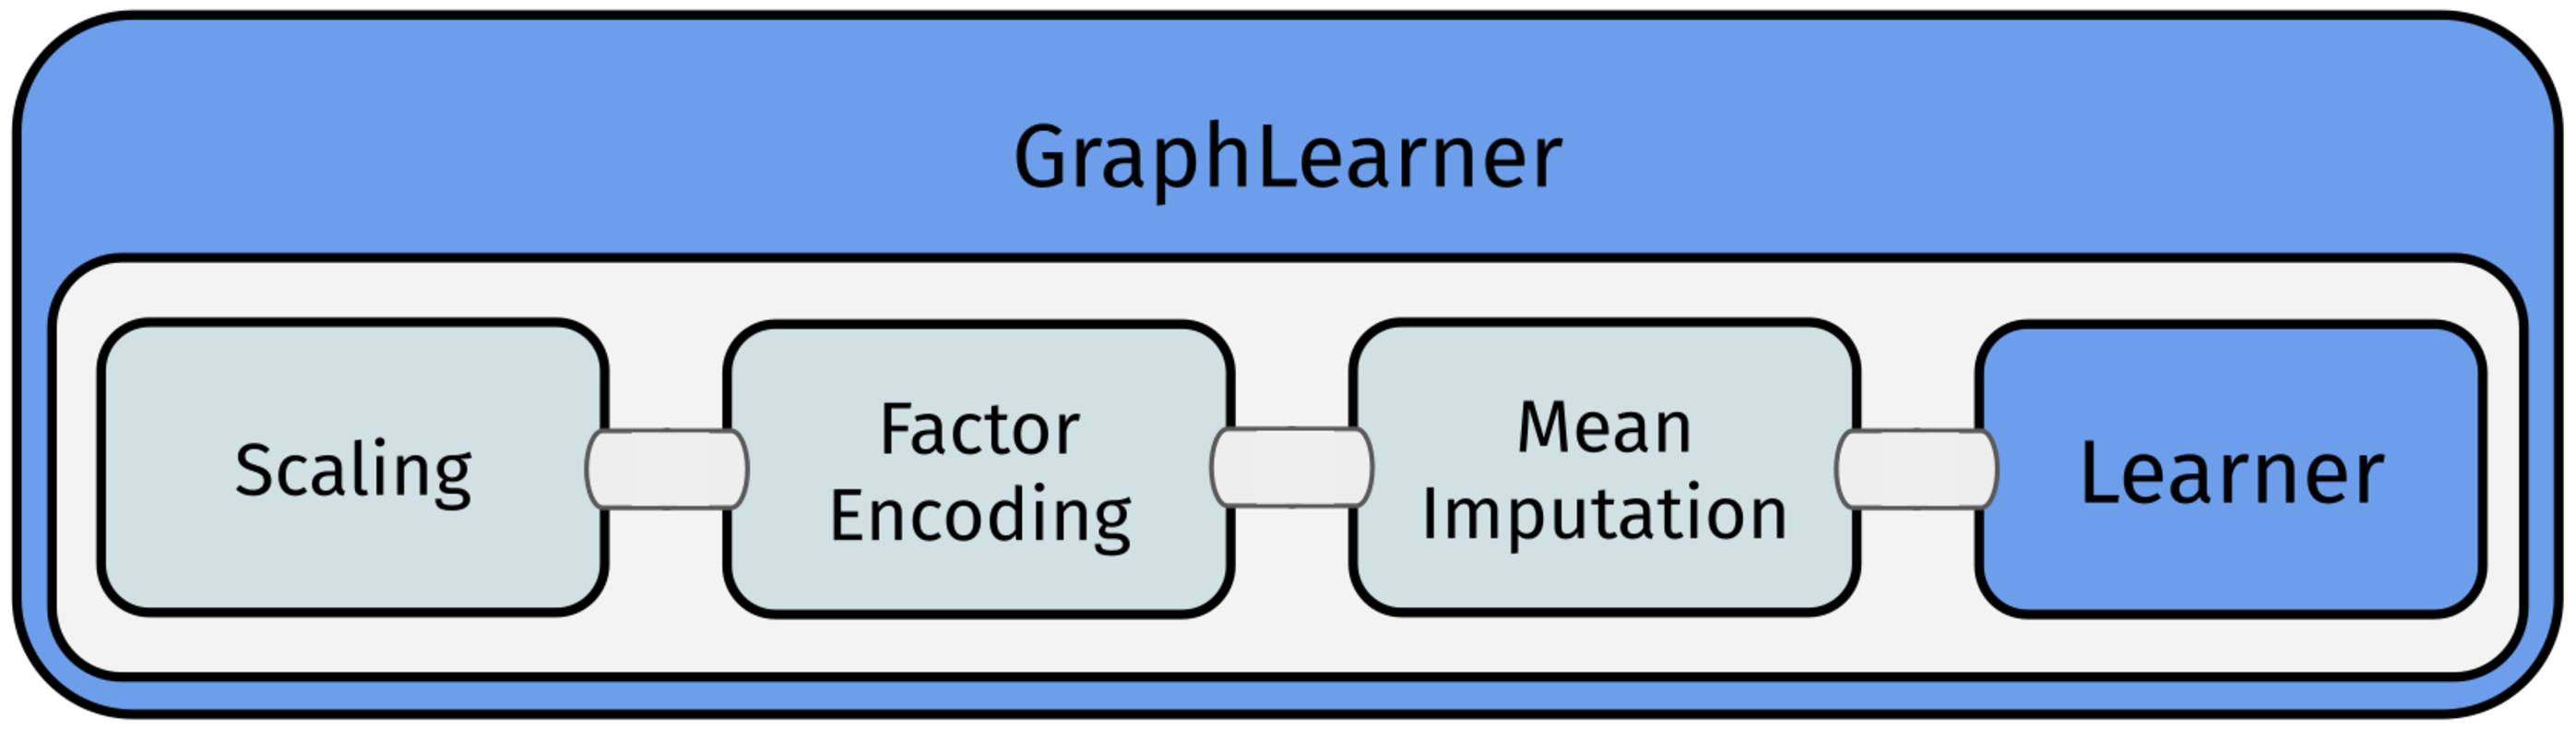
\includegraphics[width=0.7\textwidth]{img/grl_linear.pdf}
              \end{center}
              Each operation in the above example is a \codeinline{PipeOp} which transforms the data in each step. \codeinline{PipeOp}s are chained with the \codeinline{\%>{}>\%} operator.
            \end{myblock}
            \vspace{-1.0em}
            \begin{myblock}{PipeOp}
              \vspace{-1.0em}
              Flow operation with \codeinline{\$train()} and \codeinline{\$predict()} step.
              \begin{center}
                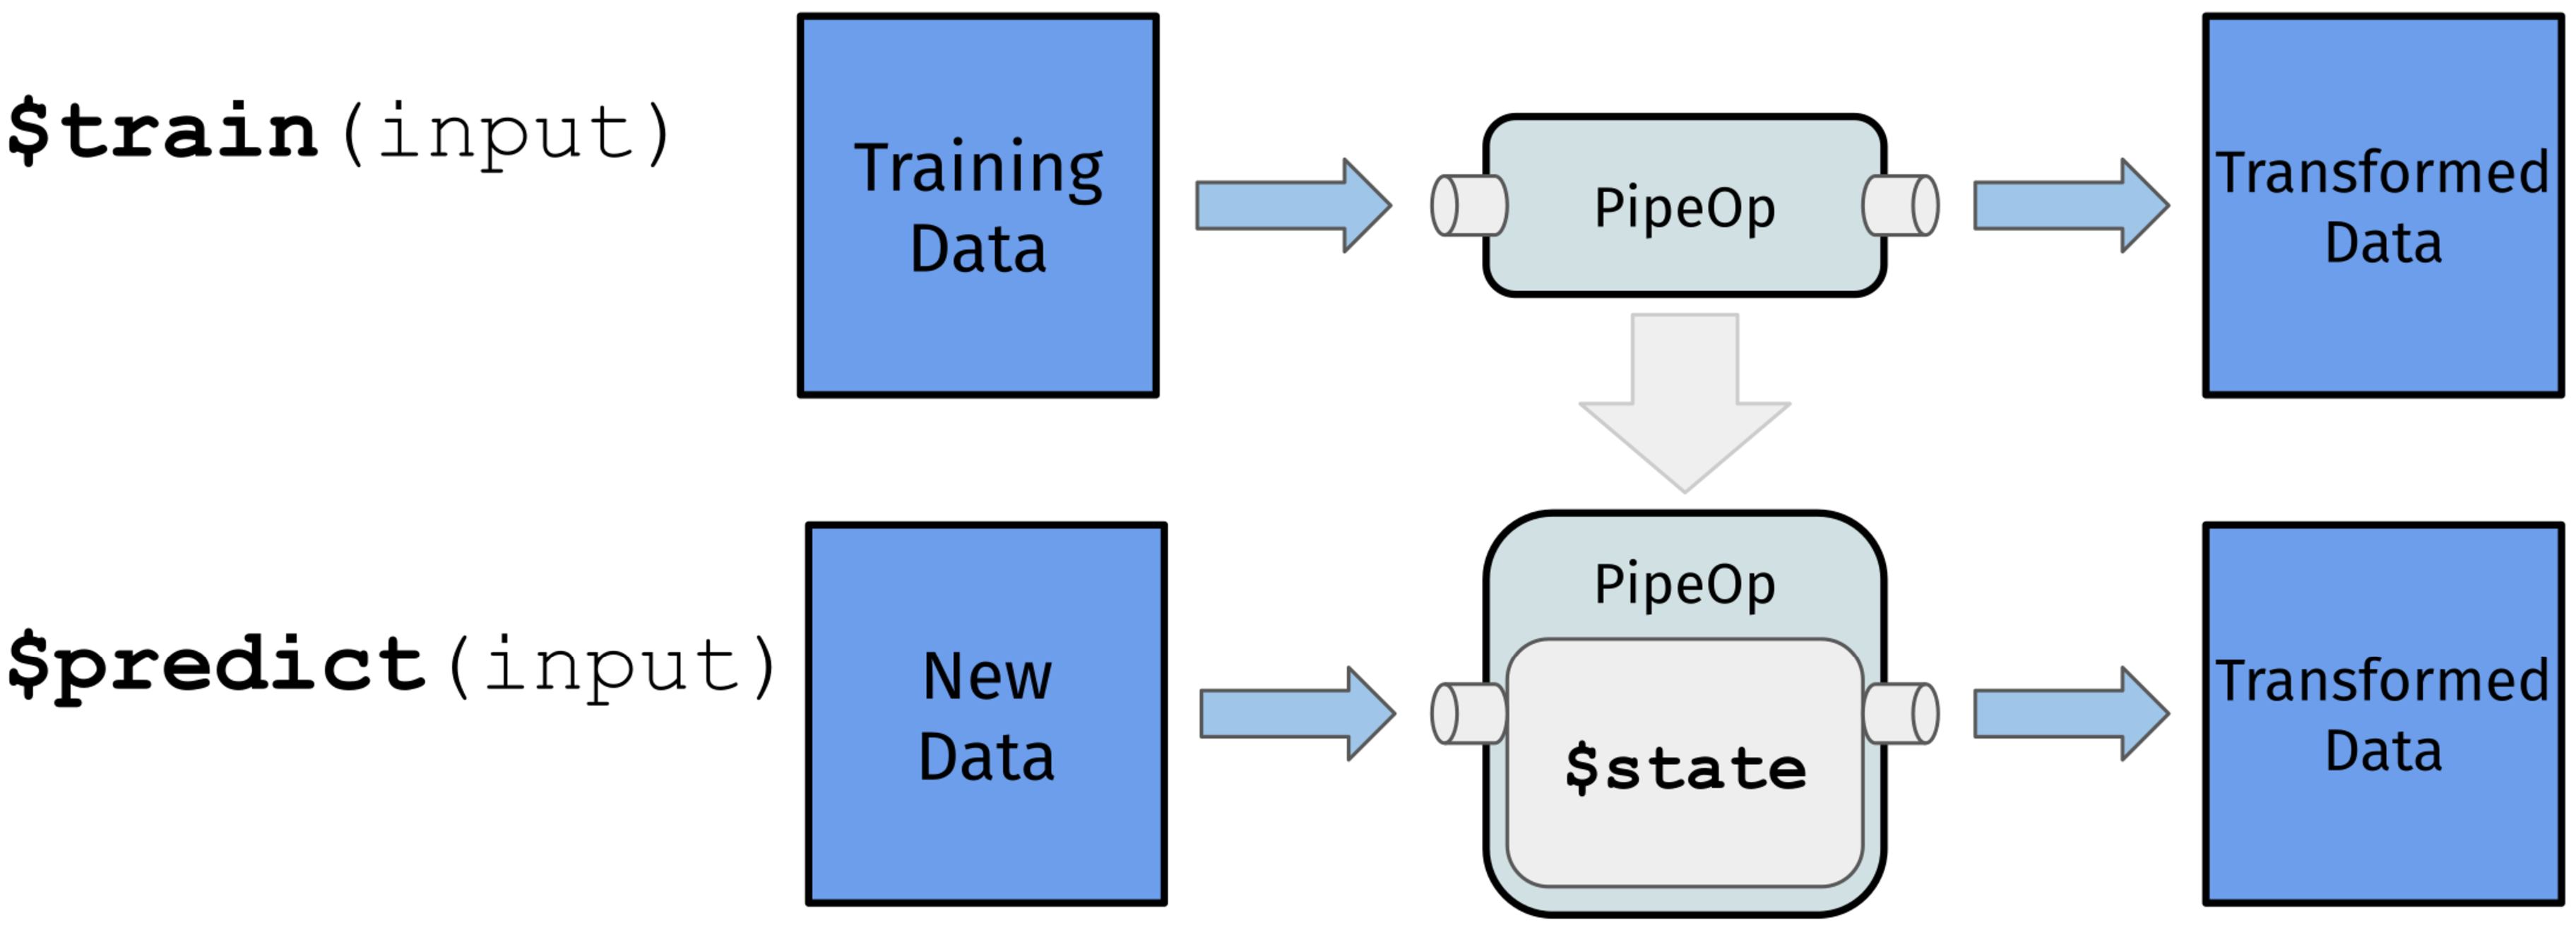
\includegraphics[width=0.7\textwidth]{img/po.pdf}
              \end{center}
              Construction example: \codeinline{pca = \textbf{po}("pca")}
              \\
              \begin{itemize}
                \item \codeinline{\textbf{\$train}(input)}: Named list
                \item \codeinline{\textbf{\$predict}(input)}: Named list
                \item \codeinline{\textbf{\$state}}: Learned parameters
                      % obtained during training and usually required for prediction
                \item \codeinline{\textbf{\$param\_set}}: See hyperparameters
              \end{itemize}
            \end{myblock}
            \vspace{-1.0em}
            \begin{myblock}{Popular PipeOps}
              \begin{footnotesize}
                \begin{centering}
                  \begin{tabular}{l l l}
                    \textbf{Class}        & \textbf{Key}      & \textbf{Operation}    \\ \hline
                    PipeOpRemoveConstants & "removeconstants" & Repair Tasks          \\
                    PipeOpScale           & "scale"           & Scale Features        \\
                    PipeOpImputeMean      & "impute"          & Impute NAs            \\
                    PipeOpFilter          & "filter"          & Feature Filter        \\
                    PipeOpEncode          & "encode"          & Factor Encoding       \\
                    PipeOpPCA             & "pca"             & PCA                   \\
                    PipeOpSelect          & "select"          & Restrict Columns      \\
                    PipeOpColApply        & "colapply"        & Transform Columns     \\
                    PipeOpClassBalancing  & "classbalancing"  & Imbalanced Data       \\
                    PipeOpLearner         & "learner"         & Use Learner           \\
                    PipeOpLearnerCV       & "learner\_cv"     & Crossval Learner      \\
                    PipeOpMutate          & "mutate"          & Fearure Engineering   \\
                    PipeOpChunk           & "chunk"           & Split Data            \\
                    PipeOpSubsample       & "subsample"       & Subsample Rows        \\
                    PipeOpFeatureUnion    & "featureunion"    & Combine Features      \\
                    PipeOpFixFactors      & "fixfactors"      & Handle Unknown Levels \\
                    PipeOpNOP             & "nop"             & Do Nothing            \\
                    \hline
                    % PipeOpChunk & "mutate" & Fearure Engineering\\ \hline
                  \end{tabular}
                \end{centering}
              \end{footnotesize}
              \ \\
              Full list: \codeinline{as.data.table(mlr\_pipeops)}
            \end{myblock}
            \vfill}
        \end{minipage}
      \end{beamercolorbox}
    \end{column}
    \begin{column}{.245\textwidth}
      \begin{beamercolorbox}[center]{postercolumn}
        \begin{minipage}{.98\textwidth}
          \parbox[t][\columnheight]{\textwidth}{
            % \vspace{-0.5em}
            \begin{myblock}{Graph}
              Connects \codeinline{PipeOp}s with edges to control data flow during training and prediction. Input is sent to sources (no in-edges), output is read from sinks (no out-edges).
              \\
              % \codeinline{PipeOp}s can have different numbers of \codeinline{\$input}s and  \codeinline{\$output}s.\\
              % Can be constructed by concatenating \codeinline{PipeOp}s via \codeinline{\%>{}>\%}, or using \codeinline{Graph\$new()}.\\
              % The return value corresponds to the output of the \codeinline{PipeOp} outputs that are not connected to other \codeinline{PipeOp}s.\\
              % Trained and predicted \codeinline{Graph} has a \codeinline{\$train()} and \codeinline{\$predict()} method that accept data and propagate this data through the network of \codeinline{PipeOp}s. The return value corresponds to the output of the \codeinline{PipeOp} outputs that are not connected to other \codeinline{PipeOp}s.\\
              % this requires the number of outputs and inputs to match:
              % \begin{codebox}
              % gr = po("pca") \textbf{\%>{}>\%} lrn("classif.rpart")
              % \end{codebox}
              \ \\
              Important methods and slots:
              \begin{itemize}
                \item Display: \codeinline{\textbf{print}(gr)}, \codeinline{gr\$\textbf{plot}(html = TRUE)}\\
                \item Accessing \codeinline{PipeOp}s: \codeinline{gr\$\textbf{pipeops}}\\
                      Named list of all contained POs.
              \end{itemize}
            \end{myblock}
            \begin{myblock}{Graph Construction}
              The \codeinline{\%>{}>\%} operator takes either a \codeinline{PipeOp} or a \codeinline{Graph} on each of its sides and connects all left-hand outputs to the right-hand inputs.
              \ \\
              \\
              For full control, connect \codeinline{PipeOp}s explicitly:
              \begin{codeboxmultiline}[width=23cm]
                gr = \textbf{Graph}\$new()\\
                gr\$\textbf{add\_pipeop}(po("pca"))\\
                gr\$\textbf{add\_pipeop}(lrn("classif.rpart"))\\
                gr\$\textbf{add\_edge}("pca", "classif.rpart")
              \end{codeboxmultiline}
            \end{myblock}
            \vspace{-0.5em}
            \begin{myblock}{GraphLearner}
              \vspace{-0.5em}
              \codeinline{GraphLearner} behave like \codeinline{Learner} and enable all mlr3 features.
              : \codeinline{grl = \textbf{GraphLearner}\$new(gr)}\\
              \\
              See slots \codeinline{\$encapsulate} for debugging and \codeinline{\$model} for results after training.
              % NB \codeinline{grl\$predict\_type} must be set exp.
            \end{myblock}
            \begin{myblock}{Linear Graphs}
              \vspace{-0.5em}
              Concatenate POs with \codeinline{\%>{}>\%}:
              \\
              % Below, we construct the introductory example: scaling, one-hot encoding and mean imputation. By wrapping the \codeinline{Graph} in a \codeinline{GraphLearner} we construct a \codeinline{Learner}.
              \begin{codeboxexample}
                {\footnotesize
                % \# construct the graph:\\
                gr = po("scale") \%>{}>\% po("encode") \%>{}>\%\\
                \hspace*{1ex} po("imputemean") \%>{}>\% lrn("classif.rpart")\\
                grl = GraphLearner\$new(gr)\\
                \# access the scale pipeop:
                grl\$graph\$pipeops\$scale\\
                % \# train and predict on a task:\\
                grl\$train(task)\\
                grl\$model\\
                grl\$predict(task)\\
                % \# perform resampling (3-fold cv):\\
                % rcv = rsmp("cv", folds = 3)\\
                % rcv\$instantiate(task)\\
                rr = resample(task, grl, rsmp("cv", folds = 3))
                }
              \end{codeboxexample}
            \end{myblock}
            \vfill}
        \end{minipage}
      \end{beamercolorbox}
    \end{column}
    \begin{column}{.245\textwidth}
      \begin{beamercolorbox}[center]{postercolumn}
        \begin{minipage}{.98\textwidth}
          \parbox[t][\columnheight]{\textwidth}{
            \begin{myblock}{Hyperparameters}
              % mlr3pipelines relies on the paradox package to provide parameters that can modify a \codeinline{PipeOp}'s or \codeinline{Graph}'s behavior. 
              For POs: Exactly as in a \codeinline{Learner}.
              \\
              % To inspect the parameters see the \codeinline{\$param\_set}, e.g., \codeinline{po("pca")\$\textbf{param\_set}}.\\
              % Access the \codeinline{\$param\_set\$values} slot to set or retrieve a parameter, or specify \codeinline{param\_vals} during construction:
              \begin{codeboxmultiline}[width=26cm]
                {\footnotesize enc = po("encode") \\
                  enc\$param\_set\\
                  enc\$param\_set\$\textbf{values} = list(method="one-hot") \\
                  % \# alternatively:\\
                  po("encode", \textbf{param\_vals} = list(method="one-hot"))}
              \end{codeboxmultiline}
              \vspace{1.0em}
              For \codeinline{Graph} / \codeinline{GraphLearner}: All HPs are collected in a global ParamSet stored in \codeinline{\$param\_set}.
              IDs are prefixed with the respective \codeinline{PipeOp}'s \codeinline{id}.
              % e.g., \codeinline{pca.rank.} corresponds to the \codeinline{PipeOpPCA}'s \codeinline{rank.} parameter.
              % . A \codeinline{GraphLearner} preserves the parameters of its encapsulated objects.\\ . A \codeinline{GraphLearner} preserves the parameters of its encapsulated objects.\\
              % \ \\
              % The parameters of all \codeinline{PipeOp}s and \codeinline{Learner}s in a \codeinline{Graph} can be jointly tuned. 
              % This can be done as with any other \codeinline{Learner} (see \href{FIXME:CheatsheetLink}{mlr3tuning}). 
              % Hyperparameter names are prefixed with the respective \codeinline{PipeOp}'s \codeinline{id}, e.g., \codeinline{pca.rank.} corresponds to the \codeinline{PipeOpPCA}'s \codeinline{rank.} parameter.
            \end{myblock}
            \vspace{-1.0em}
            \begin{myblock}{Tuning}
              Can jointly tune any Pipeline.
              \\
              % Done as with any other \codeinline{Learner} (see \href{FIXME:CheatsheetLink}{mlr3tuning}). E.g., use an \codeinline{AutoTuner} for the rank parameter of the PCA and the complexity parameter of rpart with respect to the classification error as the performance measure:
              \begin{codeboxexample}
                {\footnotesize
                % task = tsk("iris")\\
                % \# pca and rpart as GraphLearner:\\
                gr = po("encode") \%>{}>\% lrn("classif.rpart")\\
                grl = GraphLearner\$new(gr)\\
                % \# inner loop holdout:\\
                % measures = msr("classif.ce")\\
                % \# define the tuning parameters:\\
                tune\_ps = ParamSet\$new(list(\\
                \hspace*{1ex} ParamFct\$new("encode.method",\\
                \hspace*{3ex} levels = c("one-hot", "poly")),\\
                % lower = 1, upper = 4),\\
                \hspace*{1ex} ParamDbl\$new("classif.rpart.cp",\\
                \hspace*{3ex} lower = 0, upper = 0.05)\\
                ))\\
                tt = term("evals", n\_evals = 20)\\
                rs = rsmp("holdout")\\
                inst = TuningInstance\$new(task, grl, rs,\\
                \hspace*{1ex} msr("classif.ce"), tune\_ps, tt)\\
                tuner = tnr("random\_search")\\
                tuner\$tune(inst)
                % resampling\_outer = rsmp("cv", folds = 2)\\
                % rr = resample(task, at, resampling\_outer)
                }
              \end{codeboxexample}
              \vspace{1.0em}
              Usage of \codeinline{AutoTuner} is identical.
            \end{myblock}
            \vspace{-1.0em}
            \begin{myblock}{Feature Engineering}
              % \codeinline{PipeOpImpute} imputes missing data. Methods include e.g. mean, median and histogram imputation.\\
              \codeinline{PipeOpMutate} adds new features.
              This works by providing expressions in a \codeinline{list}.
              \\
              \begin{codeboxexample}
                \footnotesize{
                task = tsk("iris")\\
                % \# add new features related to the iris task:\\
                mutations = list(\\
                \hspace*{1ex} Sepal.Sum = \char`\~ \ Sepal.Length + Sepal.Width\\
                % \hspace*{1ex} Petal.Sum = \char`\~ \ Petal.Length + Petal.Width\\
                )\\
                mutate = po("mutate", param\_vals =\\
                \hspace*{1ex} list(mutation = mutations))\\
                GraphLearner\$new(mutate \%>{}>\% lrn("classif.rpart"))
                }
              \end{codeboxexample}
            \end{myblock}
            \vspace{-1.0em}
            \vfill}
        \end{minipage}
      \end{beamercolorbox}
    \end{column}
    \begin{column}{.245\textwidth}
      \begin{beamercolorbox}[center]{postercolumn}
        \begin{minipage}{.98\textwidth}
          \parbox[t][\columnheight]{\textwidth}{
            \begin{myblock}{Nonlinear Graphs}
              % Multiple input/output channels allow for nonlinear \codeinline{Graphs}, using e.g. \codeinline{gunion()} or \codeinline{greplicate()}.\\
              % \ \\
              \codeinline{\textbf{gunion}()} arranges \codeinline{PipeOp}s or \codeinline{Graph}s next to each other in a disjoint graph union.
              \\
              \begin{center}
                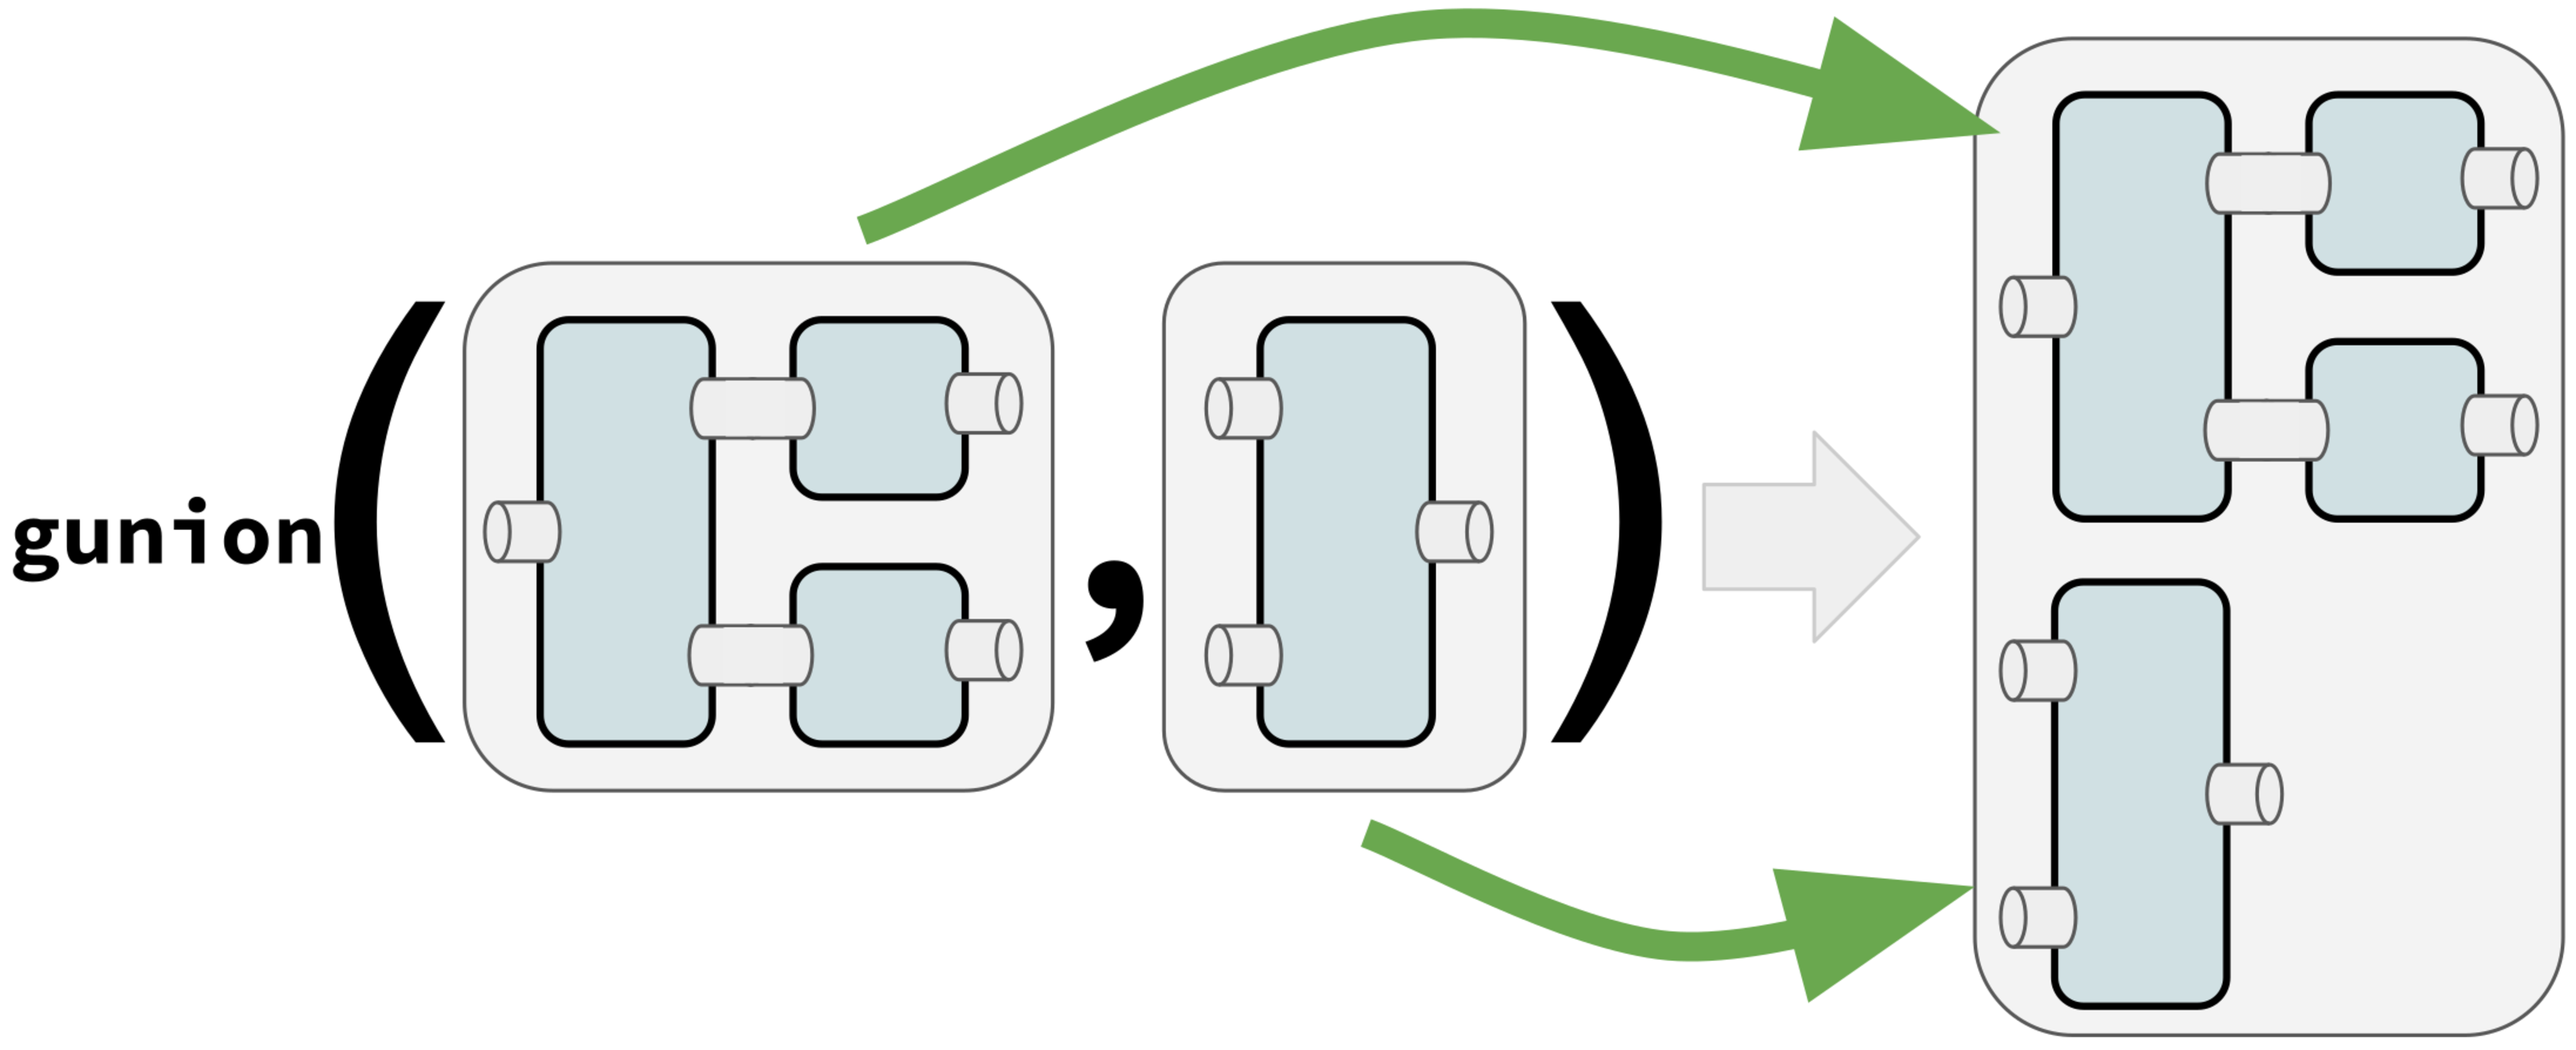
\includegraphics[width=0.7\textwidth]{img/gunion.pdf}
              \end{center}
              \vspace{0.3em}
              \codeinline{\textbf{greplicate}()} creates a new \codeinline{Graph} containing \codeinline{n} copies of the input (\codeinline{PipeOp} or \codeinline{Graph}).
              \\
              \begin{center}
                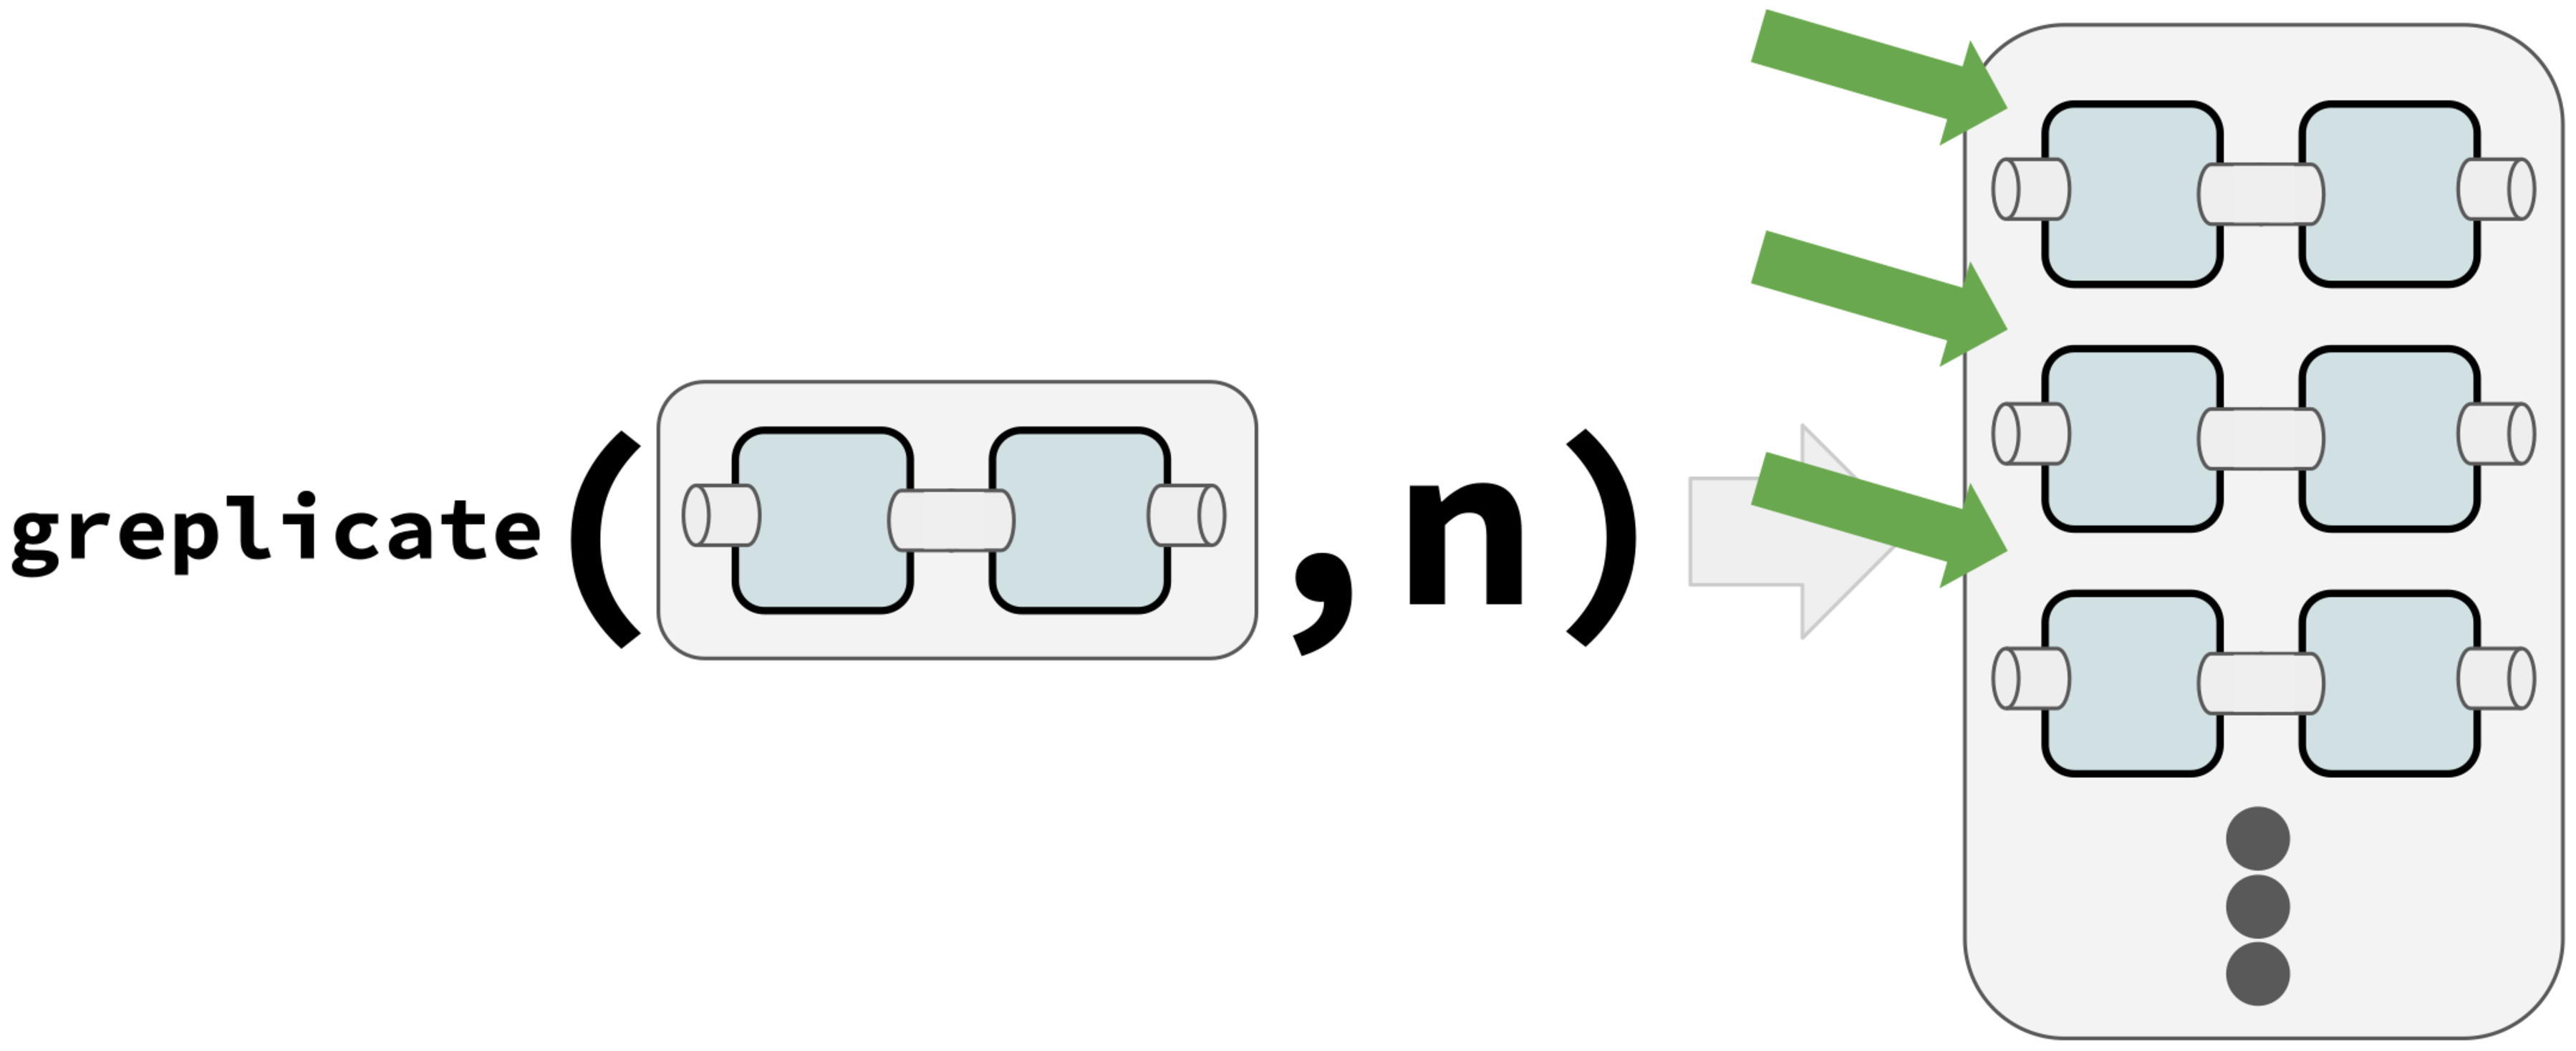
\includegraphics[width=0.7\textwidth]{img/greplicate.pdf}
              \end{center}
              \codeinline{\textbf{PipeOpFeatureUnion}} aggregates features from all input tasks into a single \codeinline{Task}.
              \\
              % (in the example below, we combine the original features obtained from \codeinline{PipeOpNOP} with the principal components obtained from \codeinline{PipeOpPCA}:
              % \vspace{0.3em}
              \begin{codeboxexample}[- Feature Union]
                {\footnotesize
                % \# copy input to nop and pca; combine the features:\\
                % gr = po("copy", outnum = 2) \%>{}>\%\\
                \# train on orig and pca features\\
                gunion(list(po("nop"), po("pca"))) \%>{}>\%\\
                po("featureunion")} \%>{}>\% lrn("classif.rpart")\\
              \end{codeboxexample}
              \begin{codeboxexample}[- Bagging Ensemble]
                {\footnotesize
                pr = po("subsample") \%>{}>\% lrn("classif.rpart")\\
                % \# 10 replicates with averaging over predictions\\
                bagging = greplicate(pr, n = 10) \%>{}>\%\\
                \hspace*{1ex} po("classifavg", innum = 10)}
              \end{codeboxexample}
            \end{myblock}
            \vspace{-1.0em}
            \begin{myblock}{Branching}
              Controls the path execution.
              Only one branch can be active.
              Which one is controlled by a hyperparameter.
              Unbranching ends the forking.
              \\
              % \codeinline{PipeOpBranch} and \codeinline{PipeOpUnbranch}, this allows for splitting a node into several paths, called \textbf{branching} (either \textit{pca} or \textit{scale} can be active):
              \begin{codeboxexample}[- Preprocessing]
                {\footnotesize
                choices = c("pca", "scale")\\
                gr = po("branch", options = choices) \%>{}>\%\\
                \hspace*{1ex} gunion(list(po("pca"), po("scale"))) \%>{}>\%\\
                \hspace*{1ex} po("unbranch", options = choices)\\
                \# set the "pca" path as the active one:\\
                gr\$param\_set\$values\$branch.selection = "pca"}
              \end{codeboxexample}
              \vspace{1.0em}
              Tuning the branching selection enables powerful model selection.
            \end{myblock}
            \vspace{-1.0em}
            \vfill}
        \end{minipage}
      \end{beamercolorbox}
    \end{column}
  \end{columns}
\end{frame}
%\begin{frame}[fragile]{}
%	\begin{columns}
%		\begin{column}{.245\textwidth}
%			\begin{beamercolorbox}[center]{postercolumn}
%				\begin{minipage}{.98\textwidth}
%					\parbox[t][\columnheight]{\textwidth}{
%           \begin{myblock}{Special PipeOps}
%             \codeinline{PipeOpImpute} imputes missing data. Methods include e.g. mean, median and histogram imputation.\\
%             \ \\
%             \codeinline{PipeOpMutate} allows for adding new features. This works by providing expressions in an \codeinline{alist}:
%             \begin{codeboxexample}
%               \footnotesize{
%               task = tsk("iris")\\
%               \# add new features related to the iris task:\\
%               mutations = list(\\
%               \hspace*{1ex} Sepal.Sum = \char`\~ \ Sepal.Length + Sepal.Width,\\
%               \hspace*{1ex} Petal.Sum = \char`\~ \ Petal.Length + Petal.Width\\
%               )\\
%               mutate = po("mutate", param\_vals =\\
%               GraphLearner\$new(mutate \%>{}>\% lrn("classif.rpart"))
%               \hspace*{1ex} list(mutation = mutations))}
%             \end{codeboxexample}
%             \ \\
%             \codeinline{PipeOpChunk} allows for splitting data into several parts.\\
%             \ \\
%             \codeinline{PipeOpFilter} can be used with filters from the mlr3filters package. Use this so select features for subsequent learners.\\
%             \ \\
%             \codeinline{PipeOpSelect} removes features from a task given a \codeinline{Selector} function defining the features to keep.
%           \end{myblock}
%         \vfill}
%				\end{minipage}
%			\end{beamercolorbox}
%		\end{column}
%    \begin{column}{.245\textwidth}
%			\begin{beamercolorbox}[center]{postercolumn}
%				\begin{minipage}{.98\textwidth}
%					\parbox[t][\columnheight]{\textwidth}{
%           \begin{myblock}{Tuning}
%             Done as with any other \codeinline{Learner} (see \href{FIXME:CheatsheetLink}{mlr3tuning}). E.g., use an \codeinline{AutoTuner} for the rank parameter of the PCA and the complexity parameter of rpart with respect to the classification error as the performance measure:
%             \begin{codeboxexample}
%						  {\footnotesize
%               task = tsk("iris")\\
%               \# pca and rpart as GraphLearner:\\
%               gr = po("pca") \%>{}>\% lrn("classif.rpart")\\
%               grl = GraphLearner\$new(gr)\\
%               \ \\
%               \# inner loop holdout:\\
%               resampling\_inner = rsmp("holdout")\\
%               measures = msr("classif.ce")\\
%               \# define the tuning parameters:\\
%               tune\_ps = ParamSet\$new(list(\\
%               \hspace*{1ex} ParamInt\$new("pca.rank.", lower = 1, upper = 4),\\
%               \hspace*{1ex} ParamDbl\$new("classif.rpart.cp",\\
%               \hspace*{2ex} lower = 0, upper = 0.05)\\
%               ))\\
%               \# 20 evaluations using grid\_search:\\
%               terminator = term("evals", n\_evals = 20)\\
%               tuner = tnr("grid\_search", resolution = 5)\\
%               \ \\
%               \# set up the auto tuner:\\
%               at = AutoTuner\$new(grl, resampling\_inner,\\
%               \hspace*{1ex} measures, tune\_ps, terminator, tuner)\\
%               \ \\
%               \# outer loop 2-fold cv:\\
%               resampling\_outer = rsmp("cv", folds = 2)\\
%               \ \\
%               rr = resample(task, at, resampling\_outer)}
%					     \end{codeboxexample}
%            \end{myblock}
%						\vfill}
%        \end{minipage}
%			\end{beamercolorbox}
%		\end{column}
%    \begin{column}{.245\textwidth}
%			\begin{beamercolorbox}[center]{postercolumn}
%				\begin{minipage}{.98\textwidth}
%					\parbox[t][\columnheight]{\textwidth}{
%            \begin{myblock}{}
%            \end{myblock}
%						\vfill}
%        \end{minipage}
%			\end{beamercolorbox}
%		\end{column}
%    \begin{column}{.245\textwidth}
%			\begin{beamercolorbox}[center]{postercolumn}
%				\begin{minipage}{.98\textwidth}
%					\parbox[t][\columnheight]{\textwidth}{
%            \begin{myblock}{}
%            \end{myblock}
%						\vfill}
%        \end{minipage}
%			\end{beamercolorbox}
%		\end{column}
%	\end{columns}
%\end{frame}
\end{document}
